\documentclass[letterpaper]{report}

\usepackage[spanish]{babel}
\usepackage[T1]{fontenc}
\usepackage{pifont}
\usepackage{pdflscape}
\usepackage{lscape}
\usepackage{geometry}
\geometry{letterpaper, margin=15mm}

%% Portada del Libro
\title{ \textbf{ \Huge Misa Italiana  } \\ { \Huge Piesas Corales } }
\author{ \textit{ \huge Pbro. Jes\'us Mar\'ia S\'anchez } } 
\date{ \LARGE Arreglo Samuel Guti\'errez \& Isabel Mart\'inez }
	
\usepackage{graphics}
\begin{document}
    
    %% - Portada
    \maketitle
     
    %% - Musica - Kyrie, eleison
    {%
\parindent 0pt
\noindent
\ifx\preLilyPondExample \undefined
\else
  \expandafter\preLilyPondExample
\fi
\def\lilypondbook{}%
\includegraphics{./07/lily-30f62566-1}%
\ifx\betweenLilyPondSystem \undefined
  \linebreak
\else
  \expandafter\betweenLilyPondSystem{1}%
\fi

\includegraphics{./07/lily-30f62566-2}%
\ifx\betweenLilyPondSystem \undefined
  \linebreak
\else
  \expandafter\betweenLilyPondSystem{2}%
\fi
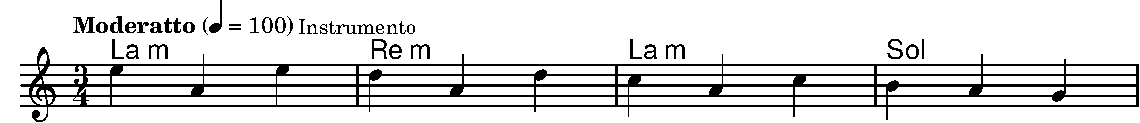
\includegraphics{./07/lily-30f62566-3}%
\ifx\betweenLilyPondSystem \undefined
  \linebreak
\else
  \expandafter\betweenLilyPondSystem{3}%
\fi
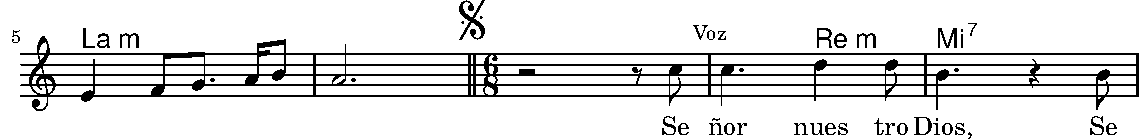
\includegraphics{./07/lily-30f62566-4}%
\ifx\betweenLilyPondSystem \undefined
  \linebreak
\else
  \expandafter\betweenLilyPondSystem{4}%
\fi
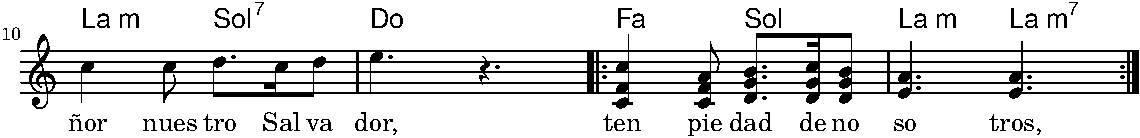
\includegraphics{./07/lily-30f62566-5}%
\ifx\betweenLilyPondSystem \undefined
  \linebreak
\else
  \expandafter\betweenLilyPondSystem{5}%
\fi
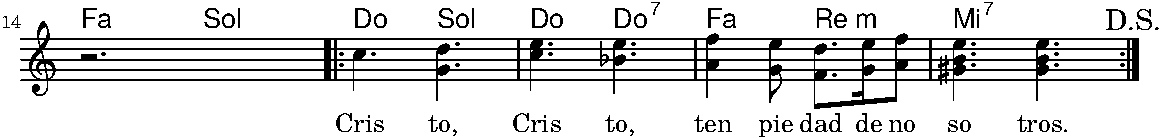
\includegraphics{./07/lily-30f62566-6}%
% eof

\ifx\postLilyPondExample \undefined
\else
  \expandafter\postLilyPondExample
\fi
}
    \clearpage
    
    %% - Musica - Gloria in excelsis Deo
    {%
\parindent 0pt
\noindent
\ifx\preLilyPondExample \undefined
\else
  \expandafter\preLilyPondExample
\fi
\def\lilypondbook{}%

\includegraphics{./c7/lily-8d3f0ae7-1}%
\ifx\betweenLilyPondSystem \undefined
  \linebreak
\else
  \expandafter\betweenLilyPondSystem{1}%
\fi
\includegraphics{./c7/lily-8d3f0ae7-2}%
\ifx\betweenLilyPondSystem \undefined
  \linebreak
\else
  \expandafter\betweenLilyPondSystem{2}%
\fi
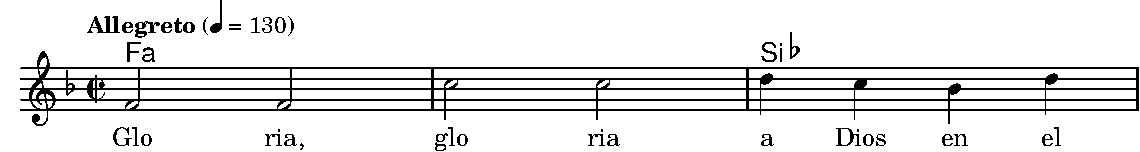
\includegraphics{./c7/lily-8d3f0ae7-3}%
\ifx\betweenLilyPondSystem \undefined
  \linebreak
\else
  \expandafter\betweenLilyPondSystem{3}%
\fi
\includegraphics{./c7/lily-8d3f0ae7-4}%
\ifx\betweenLilyPondSystem \undefined
  \linebreak
\else
  \expandafter\betweenLilyPondSystem{4}%
\fi
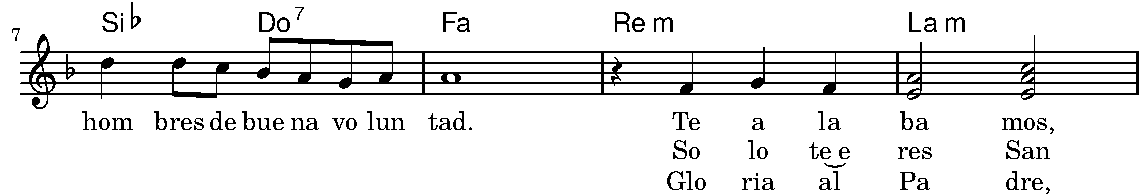
\includegraphics{./c7/lily-8d3f0ae7-5}%
\ifx\betweenLilyPondSystem \undefined
  \linebreak
\else
  \expandafter\betweenLilyPondSystem{5}%
\fi
\includegraphics{./c7/lily-8d3f0ae7-6}%
\ifx\betweenLilyPondSystem \undefined
  \linebreak
\else
  \expandafter\betweenLilyPondSystem{6}%
\fi
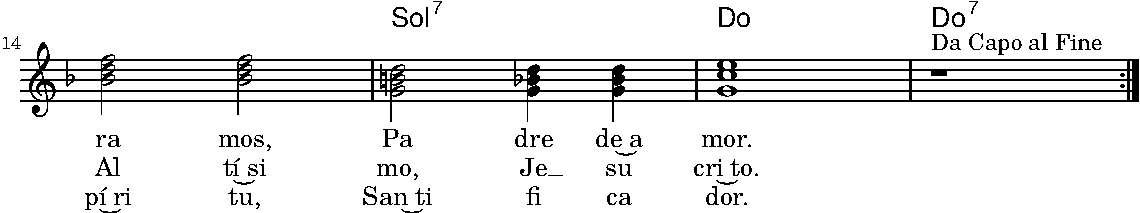
\includegraphics{./c7/lily-8d3f0ae7-7}%
\ifx\betweenLilyPondSystem \undefined
  \linebreak
\else
  \expandafter\betweenLilyPondSystem{7}%
\fi
\includegraphics{./c7/lily-8d3f0ae7-8}%
% eof

\ifx\postLilyPondExample \undefined
\else
  \expandafter\postLilyPondExample
\fi
}
    \clearpage
    
    %% - Musica - Alleluia
    {%
\parindent 0pt
\noindent
\ifx\preLilyPondExample \undefined
\else
  \expandafter\preLilyPondExample
\fi
\def\lilypondbook{}%
\includegraphics{./3c/lily-4db60daf-1}%
\ifx\betweenLilyPondSystem \undefined
  \linebreak
\else
  \expandafter\betweenLilyPondSystem{1}%
\fi
\includegraphics{./3c/lily-4db60daf-2}%
\ifx\betweenLilyPondSystem \undefined
  \linebreak
\else
  \expandafter\betweenLilyPondSystem{2}%
\fi
\includegraphics{./3c/lily-4db60daf-3}%
\ifx\betweenLilyPondSystem \undefined
  \linebreak
\else
  \expandafter\betweenLilyPondSystem{3}%
\fi
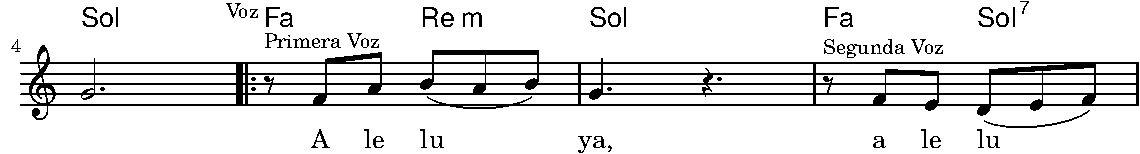
\includegraphics{./3c/lily-4db60daf-4}%
\ifx\betweenLilyPondSystem \undefined
  \linebreak
\else
  \expandafter\betweenLilyPondSystem{4}%
\fi
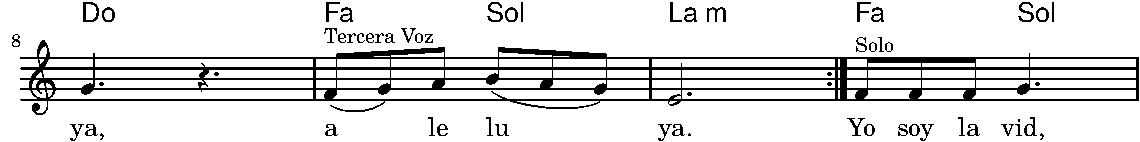
\includegraphics{./3c/lily-4db60daf-5}%
\ifx\betweenLilyPondSystem \undefined
  \linebreak
\else
  \expandafter\betweenLilyPondSystem{5}%
\fi
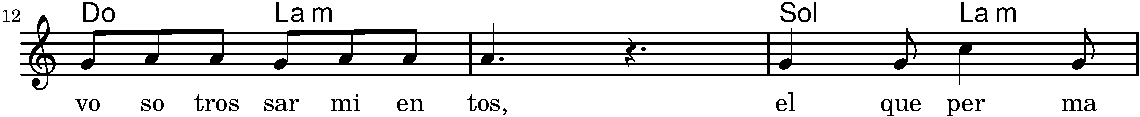
\includegraphics{./3c/lily-4db60daf-6}%
\ifx\betweenLilyPondSystem \undefined
  \linebreak
\else
  \expandafter\betweenLilyPondSystem{6}%
\fi
\includegraphics{./3c/lily-4db60daf-7}%
\ifx\betweenLilyPondSystem \undefined
  \linebreak
\else
  \expandafter\betweenLilyPondSystem{7}%
\fi
\includegraphics{./3c/lily-4db60daf-8}%
\ifx\betweenLilyPondSystem \undefined
  \linebreak
\else
  \expandafter\betweenLilyPondSystem{8}%
\fi
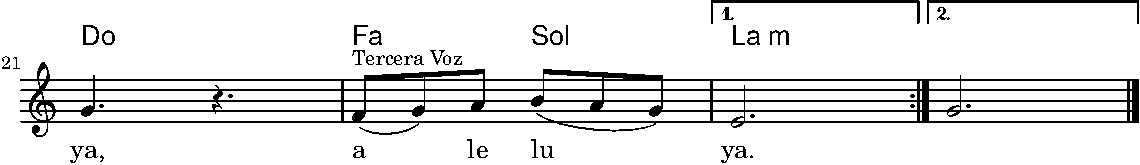
\includegraphics{./3c/lily-4db60daf-9}%
% eof

\ifx\postLilyPondExample \undefined
\else
  \expandafter\postLilyPondExample
\fi
}
    \clearpage
    
    %% - Musica - Alleluia
    {%
\parindent 0pt
\noindent
\ifx\preLilyPondExample \undefined
\else
  \expandafter\preLilyPondExample
\fi
\def\lilypondbook{}%

\includegraphics{./d4/lily-c1247149-1}%
\ifx\betweenLilyPondSystem \undefined
  \linebreak
\else
  \expandafter\betweenLilyPondSystem{1}%
\fi

\includegraphics{./d4/lily-c1247149-2}%
\ifx\betweenLilyPondSystem \undefined
  \linebreak
\else
  \expandafter\betweenLilyPondSystem{2}%
\fi
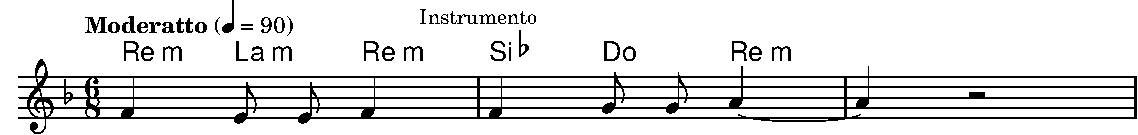
\includegraphics{./d4/lily-c1247149-3}%
\ifx\betweenLilyPondSystem \undefined
  \linebreak
\else
  \expandafter\betweenLilyPondSystem{3}%
\fi
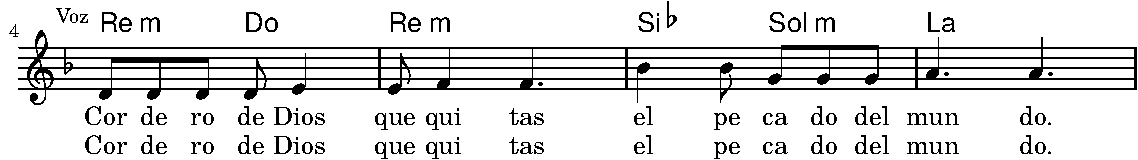
\includegraphics{./d4/lily-c1247149-4}%
\ifx\betweenLilyPondSystem \undefined
  \linebreak
\else
  \expandafter\betweenLilyPondSystem{4}%
\fi
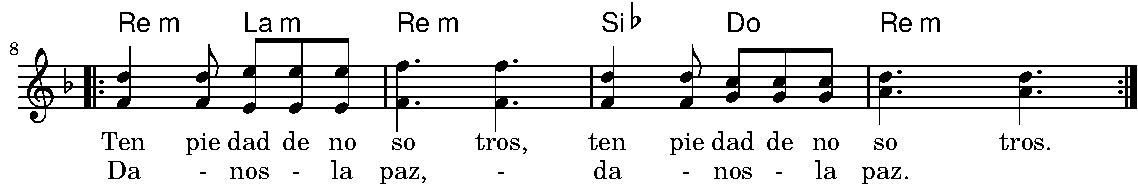
\includegraphics{./d4/lily-c1247149-5}%
% eof

\ifx\postLilyPondExample \undefined
\else
  \expandafter\postLilyPondExample
\fi
}
    \clearpage
    
\end{document}